\chapter{Risultati}
% Tabelle e grafici di ogni esperimento, con confronti fra i continual
\section{Risultati finali}
\paragraph{WESAD} Usando come modello due layer GRU da 18 unità, su WESAD sono stati ottenuti i seguenti risultati:

\begin{table}[h]
\footnotesize
    \begin{tabular}{l|c|c|c|c|c|c|c}
        \textbf{Scenario} & \textbf{Epoche} & \textbf{Tempo} & \textbf{Acc.} & \textbf{ACC} & \textbf{BWT} & \textbf{FWT} & \textbf{Memoria}\\
        \hline
        \textbf{Offline} & 28 & 94,69s & 99,07 & - & - & - & 2061,40 Mb\\
        \textbf{Continual} & 49,14$\pm$33,67 & 947,24s & 73,13$\pm$4,02 & 0,7721 & 0,0343 & 0,5397 & 2173 Mb\\
        \textbf{Cumulative} & 39,71$\pm$19,91 & 2786s & 81,97$\pm$8,67 & 0,961 & 0,1383 & 0,4674 & 2291,45 Mb\\
        \textbf{Replay} & 41,14$\pm$21,19 & 1063,51s & 78,29$\pm$3,32 & 0,7849 & -0,002 & 0,4582 & 2184,77 Mb\\
        \textbf{Episodic} & 35$\pm$26,26 & 1088,29s & 82,13$\pm$6,60 & 0,9095 & 0,0841 & 0,4226 & 2097,47 Mb\\
        \textbf{EWC} & 29,71$\pm$17,38 & 1342,81s & 70,74$\pm$4,74 & 0,7251 & 0,0113 & 0,4698 & 2187,40 Mb\\
        \textbf{LWF} & 44,29$\pm$18,30 & 3282,51s & 69,09$\pm$5,82 & 0,7419 & 0,0451 & 0,3248 & 2121,31 Mb\\
    \end{tabular}
    \caption{Risultati WESAD}
    \label{tab:reswesad}
\end{table}
\begin{figure}[h]
	\begin{center}
		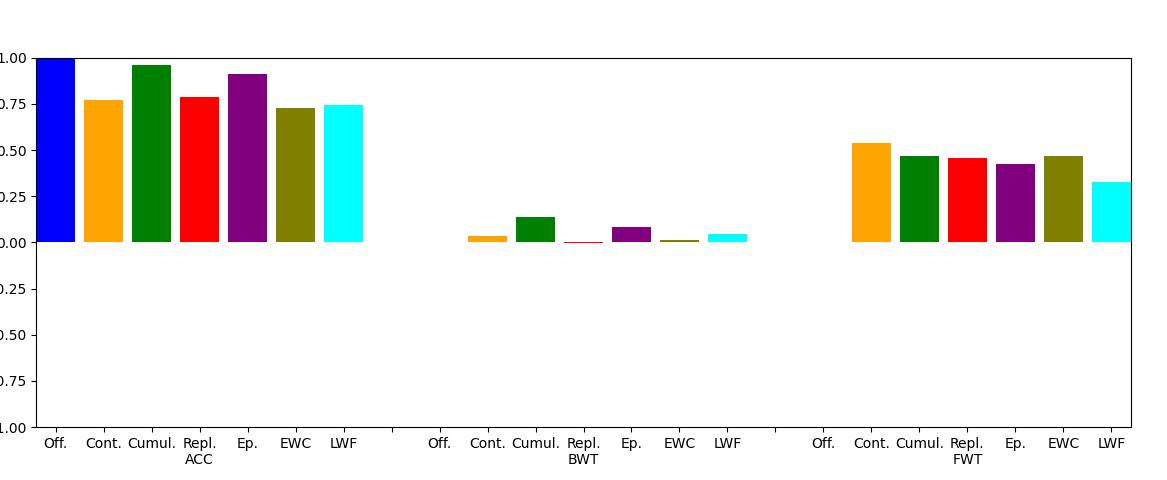
\includegraphics[width=0.95\textwidth]{img/graphs/wesad_final_metrics.png}
		\caption{Risultati su WESAD}
		\label{fig:wesad_metrics_graph}
	\end{center}
\end{figure}

L'accuratezza del 99\% raggiunta nel training offline dimostra come il dataset WESAD sia particolarmente adatto all'inferenza da parte di reti neurali ricorrenti dalla bassa complessità. Con poco più di 25 epoche di addestramento, abbiamo ottenuto un modello capace di classificare con un alto grado di accuratezza lo stato psico-fisico di un utente.\\
Ciò che è interessante notare è che l'accuratezza è mantenuta sopra il 70\% anche nella maggior parte degli approcci continual. La performance peggiore media la si ha nel \textit{Learning Without Forgetting}, che però ottiene comunque un'accuratezza finale (ACC) del 74\% e un FWT comunque ottimo. La miglior performance tra gli approcci continual è ottenuta dall'apprendimento cumulativo, con un'accuratezza finale del 96\% perfettamente paragonabile all'approccio offline, e in linea con la teoria. In tutti gli approcci, si ha un FWT elevato e molto superiore al BWT, segnale che ogni soggetto migliora molto l'apprendimento sui soggetti successivi, mentre non vi è particolare influenza sui precedenti soggetti o, se vi è, è positiva.\\\\
L'esperimento quindi dimostra come l'apprendimento continuo su dati sensoriali come respirazione, temperatura, elettrocardiogramma e simili possa portare a modelli con performance paragonabili all'apprendimento offline. Con un po' di \textit{fine-tuning} e \textit{model selection} con gli approcci continui si può probabilmente trovare un modello con performance ancora superiori a quelle sperimentate.
\begin{figure}[h]
	\begin{center}
		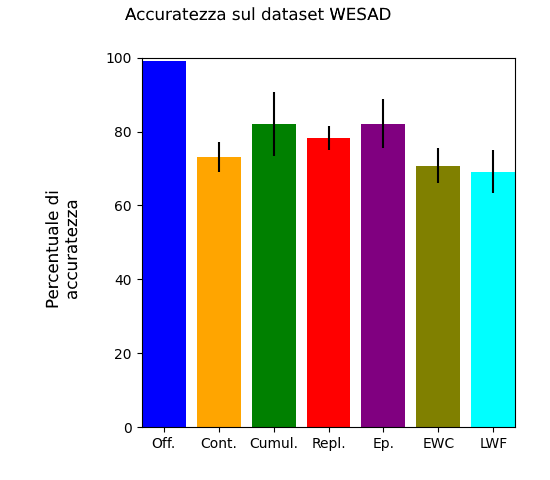
\includegraphics[width=0.65\textwidth]{img/graphs/wesad_final_accuracy.png}
		\caption{Accuratezza su WESAD}
		\label{fig:wesad_accuracy_graph}
	\end{center}
\end{figure}
\pagebreak
\paragraph{ASCERTAIN} Usando come modello due layer GRU da 24 unità, su ASCERTAIN sono stati raggiunti i seguenti risultati:
\begin{table}[h]
\footnotesize
    \begin{tabular}{l|c|c|c|c|c|c|c}
        \textbf{Scenario} & \textbf{Epoche} & \textbf{Tempo} & \textbf{Acc.} & \textbf{ACC} & \textbf{BWT} & \textbf{FWT} & \textbf{Memoria}\\
        \hline
         \textbf{Offline} & 3 & 29,14s & 42,78 & - & - & - & 1817,28 Mb\\
        \textbf{Continual} & 10,88$\pm$5,01 & 249,28s & 37,45$\pm$5,01 & 0,25 & -0,0168 & 0,0213 & 2154,36 Mb\\
        \textbf{Cumulative} & 9,25$\pm$6,81 & 932,56s & 39,06$\pm$4,26 & 0,2697 & 0,0064 & 0,0278 & 2297,17 Mb\\
        \textbf{Replay} & 13,25$\pm$10,03 & 402,96s & 39,48$\pm$4,37 & 0,2603 & -0,014 & 0,0485 & 2173,95 Mb\\
        \textbf{Episodic} & 12,62$\pm$7,94 & 498,24s & 38,80$\pm$4,04 & 0,2742 & 0,0048 & 0,0156 & 2231,42 Mb\\
        \textbf{EWC} & 24,14$\pm$16,94 & 810,96s & 36,08$\pm$5,66 & 0,2497 & -0,0183 & -0,0003 & 2171,62 Mb\\
        \textbf{LWF} & 21,62$\pm$10,20 & 879,68s & 35,69$\pm$5,43 & 0,2448 & 0.0327 & 0,0156 & 2103 Mb\\
    \end{tabular}
    \caption{Risultati ASCERTAIN}
    \label{tab:resascertain}
\end{table}
\begin{figure}[h]
	\begin{center}
		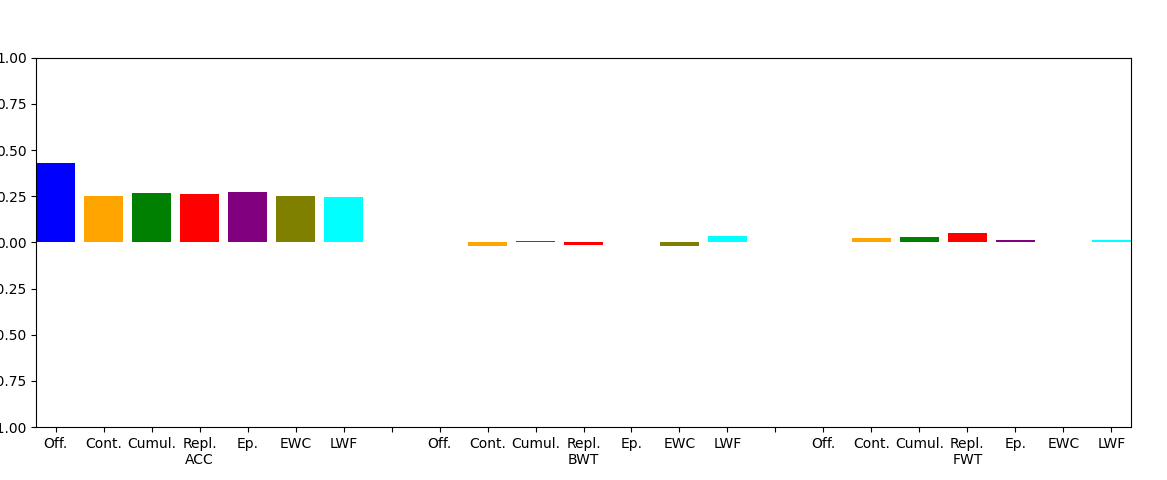
\includegraphics[width=0.95\textwidth]{img/graphs/ascertain_final_metrics.png}
		\caption{Risultati sul dataset ASCERTAIN}
		\label{fig:ascertain_metrics_graph}
	\end{center}
\end{figure}

Dall'approccio offline è subito chiaro come il dataset ASCERTAIN presenti una difficoltà maggiore rispetto a WESAD. In particolare, il dataset ASCERTAIN presenta dati particolarmente sbilanciati sulla classe 0 e informazioni riguardo le espressioni facciali dei soggetti durante l'esperimento. Questi dati sono di difficile classificazione.\\
Gli approcci continui sono comunque in linea con i risultati sul precedente dataset, con la performance peggiore ottenuta dal \textit{Learning Without Forgetting} mentre la migliore è ottenuta dall'approccio cumulativo grazie ad un BWT superiore all'approccio di replay. In molti casi si nota un trasferimento negativo di conoscenza all'indietro, sintomo di un lieve caso di \textit{catastrophic forgetting}.\\\\
Per poter dimostrare l'impatto dovuto allo sbilanciamento delle classi, il dataset ASCERTAIN è stato riorganizzato in soggetti "fittizi" come esposto di seguito.
\pagebreak
\paragraph{Custom ASCERTAIN} Dopo aver eseguito il preprocessing specificato precedentemente, tutti i dati di addestramento sono stati uniti in un unico insieme. Da questo insieme è stato estratto il test set, e il rimanente training set è stato suddiviso in 17 soggetti bilanciati da 108 sequenze di 160 punti ciascuno.\\
Usando come modello due layer GRU da 24 unità, su ASCERTAIN con i soggetti fittizi sono stati registrati i seguenti risultati:
\begin{table}[h]
\footnotesize
    \begin{tabular}{l|c|c|c|c|c|c|c}
        \textbf{Scenario} & \textbf{Epoche} & \textbf{Tempo} & \textbf{Acc.} & \textbf{ACC} & \textbf{BWT} & \textbf{FWT} & \textbf{Memoria}\\
        \hline
         \textbf{Offline} & 29 & 66,17s & 87,77 & - & - & - & 1945,91 Mb\\
        \textbf{Continual} & 7,75$\pm$5,33 & 226,24s & 87,01$\pm$0,64 & 0,2481 & -0,0241 & 0,0052 & 2143,71 Mb\\
        \textbf{Cumulative} & 7,25$\pm$8,80 & 872,8s & 87,66$\pm$0,16 & 0,2773 & 0,0032 & 0,0801 & 2273,07 Mb\\
        \textbf{Replay} & 12,125$\pm$12,94 & 299,52s & 87,13$\pm$0,75 & 0,2711 & -0,0012 & 0,306 & 2146,35 Mb\\
        \textbf{Episodic} & 5,5$\pm$3,94 & 319,76s & 82,19$\pm$3,95 & 0,339 & 0,0346 & 0,1043 & 2204,84 Mb\\
        \textbf{EWC} & 14,38$\pm$7,58 & 541,68s & 87,34$\pm$0,42 & 0,2467 & -0,0191 & 0,0845 & 2146,36 Mb\\
        \textbf{LWF} & 20,75$\pm$8,42 & 771,36s & 86,91$\pm$0,89 & 0,2495 & -0,0333 & -0,146 & 2095,93 Mb\\
    \end{tabular}
    \caption{Risultati su ASCERTAIN con soggetti fittizi bilanciati}
    \label{tab:rescustomascertain}
\end{table}
\begin{figure}[h]
	\begin{center}
		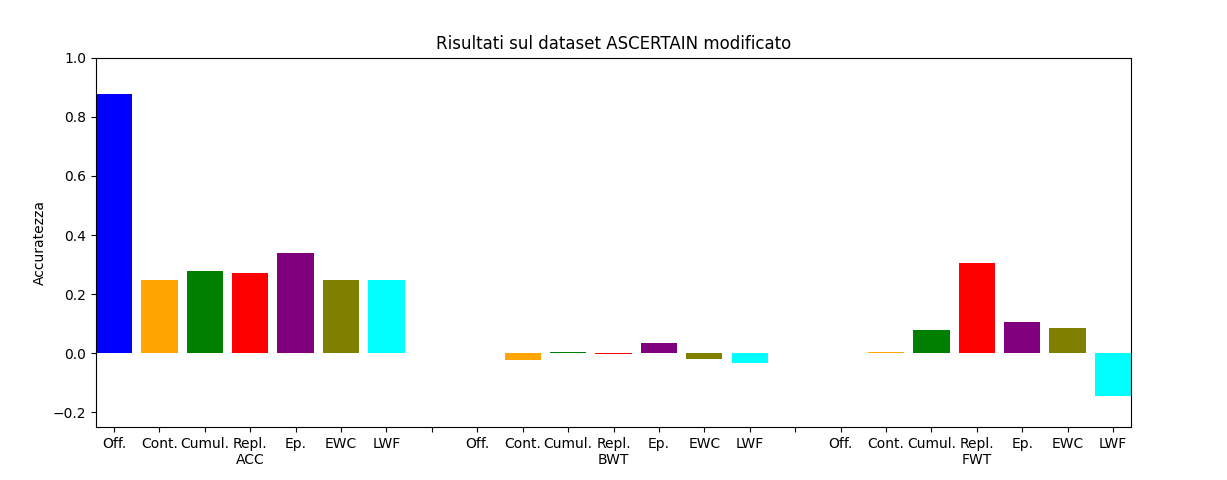
\includegraphics[width=0.95\textwidth]{img/graphs/customascertain_final_metrics.png}
		\caption{Risultati su ASCERTAIN con soggetti fittizi}
		\label{fig:customascertain_metrics_graph}
	\end{center}
\end{figure}

Dalla tabella \ref{tab:rescustomascertain} si evince subito come il bilanciamento abbia prodotto accuratezze medie molto superiori al dataset originale: l'approccio offline raggiunge l'87,77\% di accuratezza, paragonabile ai risultati ottenuti sul dataset WESAD, e gli approcci continui, in linea coi precedenti risultati, superano comunque l'80\% di accuratezza media in tutti i casi.\\
Dalle rimanenti metriche si nota comunque la difficoltà intrinseca del dataset, che raggiunge un'accuratezza finale del solo 33\% con l'approccio di replay episodico e BWT spesso negativo o comunque molto basso.
\begin{figure}[!tbp]
    \begin{minipage}[b]{0.5\textwidth}
		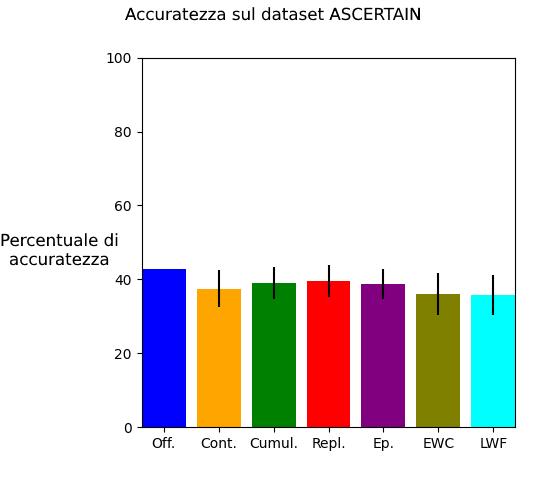
\includegraphics[width=\textwidth]{img/graphs/ascertain_final_accuracy.png}
		\caption{Accuratezza sul dataset ASCERTAIN originale}
		\label{fig:ascertain_accuracy_graph}
	\end{minipage}
    \hfill
    \begin{minipage}[b]{0.5\textwidth}
		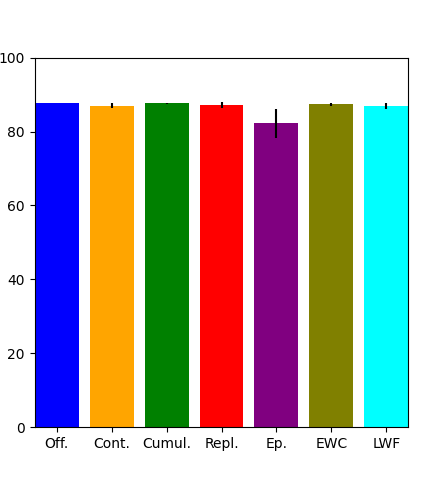
\includegraphics[width=\textwidth]{img/graphs/customascertain_final_accuracy.png}
		\caption{Accuratezza su ASCERTAIN con soggetti fittizi}
		\label{fig:customascertain_accuracy_graph}
	\end{minipage}
\end{figure}
Questa variazione del dataset ASCERTAIN dimostra come il bilanciamento dei dati di training sia fondamentale nel corretto addestramento di una rete neurale. L'avere dei soggetti di partenza bilanciati a livello di classi contenute, e di conseguenza esempi di addestramento non fortemente sbilanciati su una o più classi come nel caso del dataset ASCERTAIN originale, porta ad avere un'addestramento della rete neurale di miglior qualità e risultati finali sensibilmente migliori.